\begin{frame}[allowframebreaks]{Self Attention Layer}
    \begin{columns}
    \begin{column}{0.6\textwidth}
        \begin{figure}
            \flushleft
            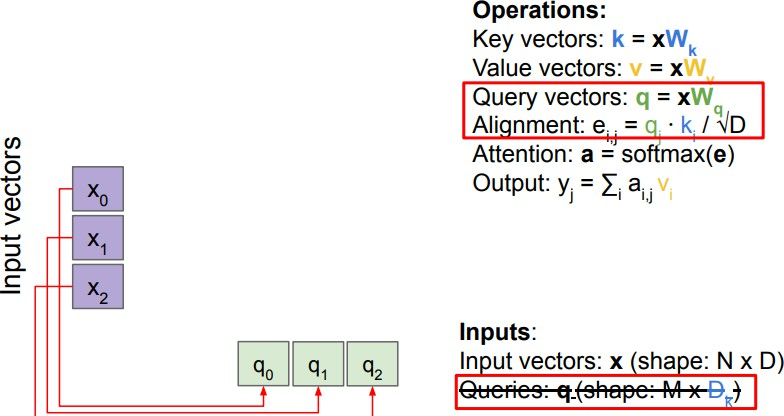
\includegraphics[width=\linewidth,height=\textheight,keepaspectratio]{images/transformers/slide_41_1_img.jpg}
        \end{figure}
    \end{column}
    \begin{column}{0.5\textwidth}
        \begin{itemize}
            \item Recall: the query vector is derived from the input vectors.
            \item In a self-attention layer, query, key, and value vectors are all computed from the same input.
            \item There are no separate input query vectors; instead, they are generated internally.
            \item Typically, fully connected (FC) layers are used to compute the query, key, and value vectors from the input.
            \item This allows each position in the input to attend to all other positions, enabling the model to capture contextual relationships.
        \end{itemize}
    \end{column}
    \end{columns}

    \framebreak

    \begin{columns}
    \begin{column}{0.6\textwidth}
        \begin{figure}
            \flushleft
            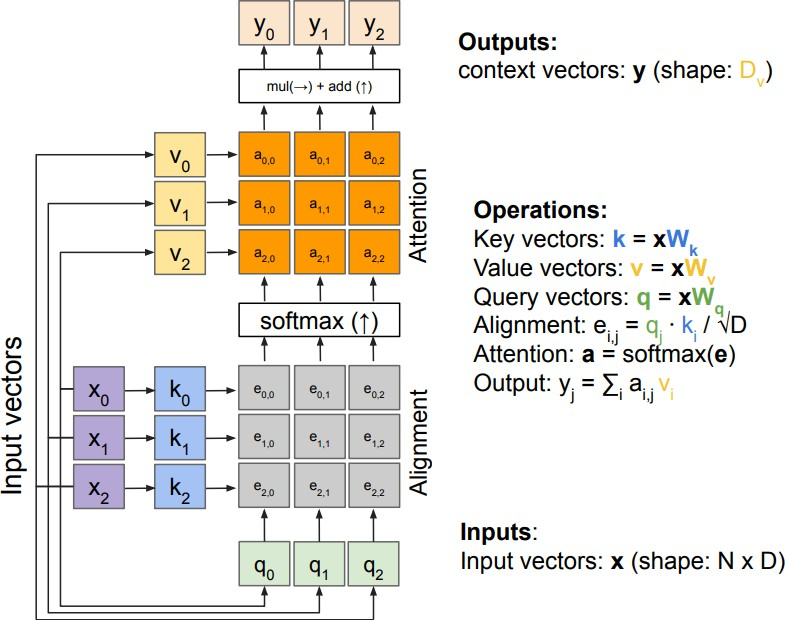
\includegraphics[width=\linewidth,height=\textheight,keepaspectratio]{images/transformers/slide_42_1_img.jpg}
        \end{figure}
    \end{column}
    \begin{column}{0.5\textwidth}
        \begin{itemize}
            \item Recall: the query vector is derived from the input vectors.
            \item In a self-attention layer, query, key, and value vectors are all computed from the same input.
            \item There are no separate input query vectors; instead, they are generated internally.
            \item Typically, fully connected (FC) layers are used to compute the query, key, and value vectors from the input.
            \item This allows each position in the input to attend to all other positions, enabling the model to capture contextual relationships.
        \end{itemize}
    \end{column}
    \end{columns}

    \framebreak

    \begin{columns}
    \begin{column}{0.7\textwidth}
        \begin{figure}
            \flushleft
            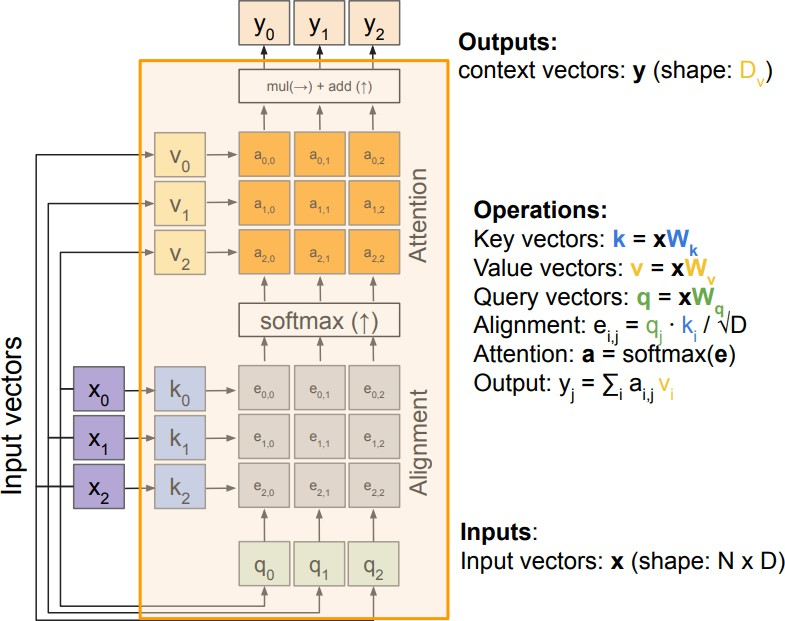
\includegraphics[width=\linewidth,height=\textheight,keepaspectratio]{images/transformers/slide_43_1_img.jpg}
        \end{figure}
    \end{column}
    \begin{column}{0.4\textwidth}
        \begin{figure}
            \centering
            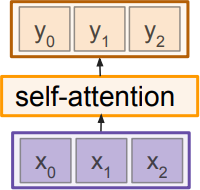
\includegraphics[width=0.8\linewidth,height=\textheight,keepaspectratio]{images/transformers/slide_43_2_img.png}
        \end{figure}
    \end{column}
    \end{columns}
\end{frame}


\begin{frame}[allowframebreaks]{Permutation Invariance}
    \begin{figure}
        \centering
        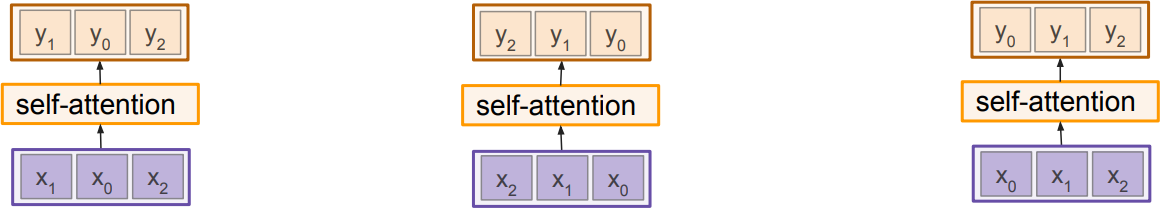
\includegraphics[width=\linewidth,height=\textheight,keepaspectratio]{images/transformers/slide_44_1_img.png}
    \end{figure}

    \vspace{1em}

    \begin{itemize}
        \item The self-attention layer is \textbf{permutation equivariant}: it produces the same output regardless of the order of the input elements.
        \item This means the model does not inherently capture the order of the sequence.
        \item \textbf{Challenge:} For tasks involving ordered data, such as language or images, we need a way to encode positional information.
        \item \textit{How can we enable the model to distinguish between different positions in a sequence?}
    \end{itemize}
\end{frame}